\section{Tìm hiểu công cụ Power BI}
\label{sec:intro_pbi}

Trong phần này, chúng tôi trình bày các kiến thức lý thuyết cơ bản và các chức năng cốt lõi của công cụ Power BI dựa trên quá trình nghiên cứu thực tế.

\subsection{Giới thiệu tổng quan về Power BI}
Power BI là một giải pháp phân tích kinh doanh (Business Intelligence) của Microsoft, cho phép người dùng trực quan hóa dữ liệu và chia sẻ thông tin chi tiết (insights) trong toàn tổ chức hoặc nhúng chúng vào ứng dụng hoặc trang web. Power BI giúp kết nối hàng trăm nguồn dữ liệu khác nhau, làm sạch và chuẩn bị dữ liệu bằng các công cụ tích hợp, sau đó tạo ra các báo cáo đẹp mắt và trực quan.

\subsection{Các thành phần chính của Power BI}
Power BI bao gồm ba thành phần chính, phối hợp chặt chẽ với nhau để tạo ra và phân phối báo cáo:
\begin{enumerate}
    \item \textbf{Power BI Desktop}: Ứng dụng miễn phí chạy trên hệ điều hành Windows, dùng để kết nối, biến đổi và trực quan hóa dữ liệu. Đây là môi trường làm việc chính của các nhà phát triển dữ liệu để xây dựng data model và tạo biểu đồ.
    \item \textbf{Power BI Service}: Dịch vụ đám mây (SaaS - Software as a Service) của Microsoft. Sau khi tạo báo cáo trên Power BI Desktop, người dùng sẽ xuất bản (publish) lên Power BI Service để chia sẻ, phân quyền, cấu hình làm mới dữ liệu tự động và xây dựng các Dashboard tổng hợp.
    \item \textbf{Power BI Mobile}: Ứng dụng trên các thiết bị di động (iOS, Android) giúp người dùng và các nhà quản lý xem các báo cáo và dashboard mọi lúc mọi nơi dưới giao diện được tối ưu hóa cho màn hình cảm ứng.
\end{enumerate}

\subsection{Các chức năng cơ bản của Power BI}
Quá trình làm việc trên Power BI thường tuân theo một quy trình chuẩn hóa gồm các chức năng cốt lõi sau:
\begin{itemize}
    \item \textbf{Import dữ liệu (Data Ingestion)}: Hỗ trợ kết nối với nhiều nguồn dữ liệu đa dạng như file tĩnh (Excel, CSV, JSON), cơ sở dữ liệu quan hệ (SQL Server, MySQL, PostgreSQL), dịch vụ đám mây (Google Analytics, Salesforce), và các API web.
    \item \textbf{Data Transformation (Power Query)}: Môi trường trực quan để làm sạch và biến đổi dữ liệu. Người dùng có thể xóa cột, lọc dòng, thay thế giá trị trống, gộp bảng (Merge Queries), hoặc nối bảng (Append Queries) mà không cần viết mã SQL phức tạp. Mọi thao tác được lưu lại dưới dạng các bước thực hiện (Applied Steps) để tự động chạy lại khi dữ liệu nguồn thay đổi.
    \item \textbf{Mô hình hóa dữ liệu (Data Modeling)}: Thiết lập mối quan hệ (relationship) giữa các bảng dựa trên các khóa chung. Tạo các cột tính toán (Calculated Columns) và các thước đo (Measures) bằng ngôn ngữ công thức DAX (Data Analysis Expressions) để thực hiện các phép toán phức tạp.
    \item \textbf{Trực quan hóa (Visualization)}: Cung cấp hàng chục loại biểu đồ mặc định (biểu đồ cột, biểu đồ đường, biểu đồ tròn, bản đồ địa lý, bảng, thẻ thông tin...) và hàng trăm biểu đồ tùy chỉnh từ thư viện AppSource để chuyển đổi các con số khô khan thành thông tin dễ hiểu.
    \item \textbf{Dashboard và Storyboard}: Kết hợp các biểu đồ quan trọng nhất từ nhiều báo cáo khác nhau lên một trang duy nhất để người quản trị có cái nhìn toàn cảnh. Thiết lập các bộ lọc (Slicers, Filters) tương tác và liên kết các trang báo cáo để tạo ra một câu chuyện mạch lạc (Storyboard) về luồng phân tích dữ liệu.
\end{itemize}

\subsection{Minh họa chức năng bằng dữ liệu mẫu}
Để làm quen với quy trình trên, nhóm đã thực hiện thử nghiệm trên một bộ dữ liệu đơn giản (\href{https://drive.google.com/drive/folders/15G17ukMnO5SE3tEGr7q1lfL1cEJYrSk0?usp=drive_link}{bộ dữ liệu mẫu Financials tích hợp sẵn trong Power BI}). Các bước thực hiện bao gồm:
\begin{enumerate}
    \item Nạp bảng dữ liệu \texttt{financials} vào Power BI Desktop.
    \item Dùng Power Query xóa các dòng trống và ép kiểu cột \texttt{Date} về định dạng \texttt{Date}.
    \item Tạo một measure tính tổng doanh thu bằng DAX: \texttt{Total Sales = SUM(financials[Sales])}.
    \item Vẽ biểu đồ cột hiển thị doanh thu theo từng tháng và biểu đồ tròn thể hiện cơ cấu sản phẩm bán ra.
\end{enumerate}

\begin{figure}[H]
    \centering
    \begin{subfigure}{0.48\textwidth}
        \centering
        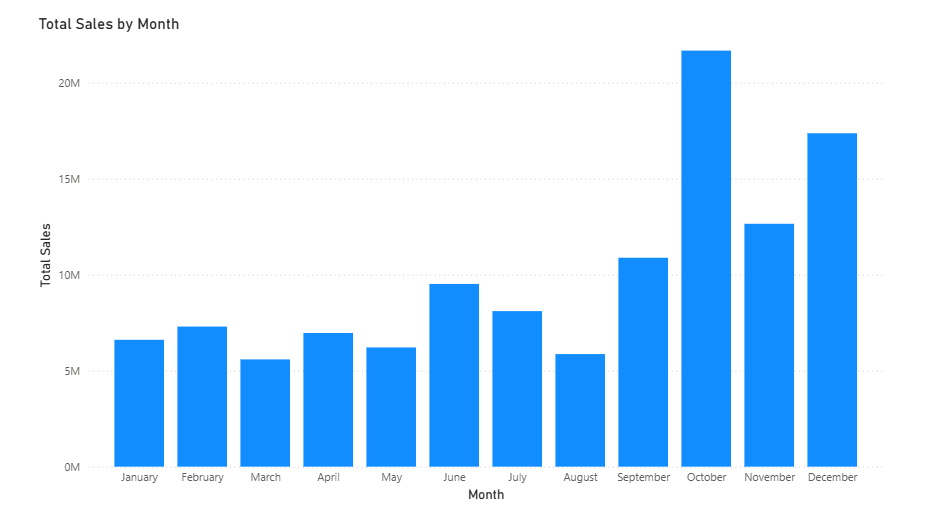
\includegraphics[width=\textwidth, keepaspectratio]{images/sample_sales_by_month.png}
        \caption{Biểu đồ cột (Doanh thu theo Tháng)}
    \end{subfigure}
    \hfill
    \begin{subfigure}{0.48\textwidth}
        \centering
        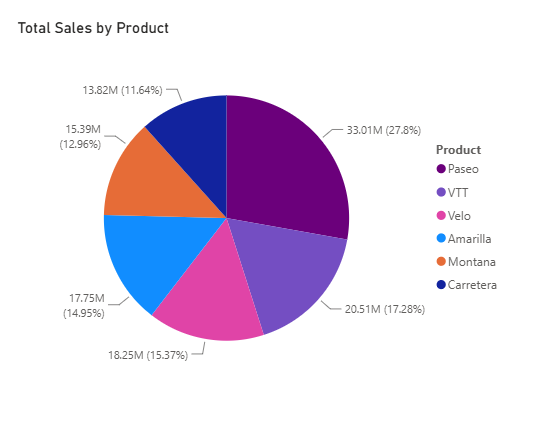
\includegraphics[width=\textwidth, keepaspectratio]{images/sample_sales_by_product.png}
        \caption{Biểu đồ tròn (Cơ cấu theo Sản phẩm)}
    \end{subfigure}
    \caption{Minh họa các biểu đồ cơ bản trên dữ liệu mẫu Financials}
    \label{fig:sample_viz}
\end{figure}

Kết quả thử nghiệm cho thấy Power BI có tốc độ xử lý nhanh, khả năng kéo thả trực quan và đồng bộ hóa bộ lọc tốt giữa các biểu đồ. Đây là tiền đề để nhóm áp dụng vào bộ dữ liệu chính của đồ án.
